\subsection{问题三模型的建立与求解}

\subsubsection{长期边界与烘干判据}

问题三保持药材半径$R_0$不变，温度场和含水率场沿用式\eqref{eq:q2-variable-heat}、式\eqref{eq:q2-variable-moisture}及附录3物性函数。附件1在$t\le t_a$内给出环境状态
\[
\boldsymbol y_a(t)=\bigl(T_a(t),C_a(t)\bigr),
\qquad t_a=4\,\mathrm h.
\]
长期边界取附件1末一小时测量值的算术平均，以减弱单个测点的波动。记该时段的测点集合为$\mathcal I=\{j:t_a-\Delta_a\le t_j\le t_a\}$，其中$\Delta_a=1\,\mathrm h$，则
\begin{equation}
\overline T_a=\frac{1}{|\mathcal I|}\sum_{j\in\mathcal I}T_a(t_j),
\qquad
\overline C_a=\frac{1}{|\mathcal I|}\sum_{j\in\mathcal I}C_a(t_j),
\qquad
\overline{\boldsymbol y}_a=(\overline T_a,\overline C_a).
\label{eq:q3r-environment-mean}
\end{equation}
记附件末值为$\boldsymbol y_a=\boldsymbol y_a(t_a)$，用过渡时间$\tau=60\,\mathrm s$将其连接至均值，得到
\begin{equation}
\boldsymbol y_\infty(t)=
\begin{cases}
\boldsymbol y_a(t),&0\le t\le t_a,\\
(1-s)\boldsymbol y_a+s\overline{\boldsymbol y}_a,
&t_a<t<t_a+\tau,\\
\overline{\boldsymbol y}_a,&t\ge t_a+\tau,
\end{cases}
\qquad s=\dfrac{t-t_a}{\tau}.
\label{eq:q3r-environment}
\end{equation}
% 待数值同步：本次将长期边界改为末一小时原始测点均值。
% 下文既有时长、表格与收敛证据采用修改前的边界，须以本式复算后更新。

定义全域最大含水率
\begin{equation}
G_3(t)=\max_{0\le r\le R_0}C(r,t),
\label{eq:q3r-maximum}
\end{equation}
则烘干临界时刻为
\begin{equation}
\boxed{
t_3=\inf\{t>0:G_3(t)<C_{\mathrm{lim}}\},
\qquad C_{\mathrm{lim}}=0.15\,\mathrm{kg/kg}.
}
\label{eq:q3r-event}
\end{equation}
计算表明$C(r,t)$随$r$单调递减，因而$G_3(t)=C(0,t)$，最终时长由圆柱中心控制。

\subsubsection{数值求解与结果}

令$x=r/R_0$，将计算域化为$x\in[0,1]$。空间上采用圆柱坐标有限体积法，并在表面含水率梯度较大的区域加密；时间上采用隐式BDF格式\cite{hairer1996}。联立求解温度场与含水率场，并由$G_3(t)-C_{\mathrm{lim}}$的零点确定$t_3$。

临界时刻为
\begin{equation}
\boxed{
t_3=206900.2366\,\mathrm s
=57.4722880\,\mathrm h.
}
\label{eq:q3r-result}
\end{equation}
计入网格加密得到的时刻误差后，第四位小数保持稳定，故第三问报告
\begin{equation}
\boxed{t_3=57.4723\,\mathrm h.}
\label{eq:q3r-reported}
\end{equation}
典型时刻的径向含水率见表\ref{tab:q3r-moisture}。

\begin{table}[H]
\centering
\renewcommand{\arraystretch}{1.15}
\caption{固定半径条件下的径向含水率}
\label{tab:q3r-moisture}
\begin{tabularx}{0.90\textwidth}{|>{\centering\arraybackslash}p{0.18\textwidth}|*{5}{>{\centering\arraybackslash}X|}}
\hline
\multirow{2}{*}{时间/h}&\multicolumn{5}{c|}{到药材中心的距离/cm}\\
\cline{2-6}
&0&0.5&1.0&1.5&2.0\\
\hline
6&1.0170&0.9881&0.9015&0.7550&0.5328\\
\hline
12&0.4561&0.4432&0.4031&0.3297&0.1642\\
\hline
18&0.2988&0.2915&0.2687&0.2253&0.0845\\
\hline
24&0.2378&0.2327&0.2167&0.1855&0.0665\\
\hline
30&0.2058&0.2018&0.1892&0.1641&0.0598\\
\hline
36&0.1859&0.1825&0.1718&0.1504&0.0566\\
\hline
42&0.1721&0.1691&0.1597&0.1407&0.0549\\
\hline
48&0.1618&0.1592&0.1507&0.1334&0.0537\\
\hline
54&0.1539&0.1514&0.1436&0.1277&0.0530\\
\hline
57.4723&0.1500&0.1477&0.1402&0.1249&0.0527\\
\hline
\end{tabularx}
\end{table}

表\ref{tab:q3r-moisture}显示，表面含水率较早接近环境水平，中心含水率下降最慢。末行的$0.1500$为显示值，式\eqref{eq:q3r-event}使用未舍入数值判断。

\subsubsection{结果检验}

取三级空间尺度$h,\,h/2,\,h/4$，以$Q_h$表示相应离散结果。观测阶和细网格余量采用\cite{roache1998}
\begin{equation}
p=\log_2\frac{|Q_h-Q_{h/2}|}{|Q_{h/2}-Q_{h/4}|},
\qquad
\varepsilon_Q=1.5\frac{|Q_{h/2}-Q_{h/4}|}{2^p-1}.
\label{eq:q3r-convergence}
\end{equation}
空间加密得到$p=2.0003$、$\varepsilon_{t,s}=0.0353\,\mathrm s$；时间加密得到$p=1.9260$、$\varepsilon_{t,t}=1.63\times10^{-4}\,\mathrm s$。计入零点定位后，临界时刻的综合经验误差为
\begin{equation}
\varepsilon_t=0.0355\,\mathrm s<0.18\,\mathrm s,
\label{eq:q3r-time-error}
\end{equation}
其中$0.18\,\mathrm s$是以小时保留四位小数的半单位，式\eqref{eq:q3r-reported}由此得到数值精度支持。

采用Chebyshev谱元--Radau方法\cite{trefethen2000,hairer1996}复算同一径向模型，所得临界时刻为$57.4722815\,\mathrm h$，与有限体积结果相差$0.0234\,\mathrm s$。进一步建立二维轴对称有限元模型\cite{hughes1987}：端面绝热、不透湿时与一维结果相差$0.1234\,\mathrm s$；端面采用侧面传递系数时，临界时刻提前$7.4619\,\mathrm s$。端面系数缺少独立测量，正文采用一维径向模型作为主模型，二维结果用于衡量端面条件的敏感性。

% 第三问数值证据：
% problem3/q3_3algo/home/zyf/CUMCM/q3/problem3_fine/validation_report.md
% problem3/q3_3algo/home/zyf/CUMCM/q3/q3q4more/experiments_spectral/Q3/comparison_report.json
% problem3/q3_3algo/home/zyf/CUMCM/q3/q3q4more/experiments_fem2d/Q3/comparison_report.json

\subsection{问题四模型的建立与求解}

\subsubsection{均匀仿射收缩主模型}

附件2给出半径序列$\{(t_j,R_j)\}$。在相邻测点之间取
\begin{equation}
R(t)=R_j+\frac{t-t_j}{t_{j+1}-t_j}(R_{j+1}-R_j),
\qquad t_j\le t\le t_{j+1}.
\label{eq:q4r-radius}
\end{equation}
式\eqref{eq:q4r-radius}描述测点间的局部变化，完整收缩曲线仍由附件2确定。

主模型假设长度保持$L_0$，各材料层具有相同的径向缩放比。初始位置$r_0$在时刻$t$运动至
\begin{equation}
r(t)=\lambda(t)r_0,
\qquad
\lambda(t)=\frac{R(t)}{R_0}.
\label{eq:q4r-affine}
\end{equation}
取材料坐标$x=r/R(t)=r_0/R_0$，并记
\[
\Theta(x,t)=T(xR(t),t),
\qquad W(x,t)=C(xR(t),t).
\]
材料速度为$u_r=(\dot R/R)r$，故材料导数满足
\begin{equation}
\frac{\mathrm Df}{\mathrm Dt}
=\left.\frac{\partial f}{\partial t}\right|_r
+u_r\frac{\partial f}{\partial r}
=\left.\frac{\partial \widehat f}{\partial t}\right|_x.
\label{eq:q4r-material-derivative}
\end{equation}
将附录4给出的物性函数记为$\rho_4(C)$、$c_{p,4}(C)$、$k_4(C)$和$D_4(C,T_K)$，则固定区间$x\in[0,1]$上的方程为
\begin{equation}
\rho_4(W)c_{p,4}(W)\frac{\partial\Theta}{\partial t}
=\frac{1}{R(t)^2x}\frac{\partial}{\partial x}
\left[xk_4(W)\frac{\partial\Theta}{\partial x}\right],
\label{eq:q4r-heat}
\end{equation}
\begin{equation}
\frac{\partial W}{\partial t}
=\frac{1}{R(t)^2x}\frac{\partial}{\partial x}
\left[xD_4(W,\Theta_K)\frac{\partial W}{\partial x}\right].
\label{eq:q4r-moisture}
\end{equation}
初始条件沿用前文，环境状态取式\eqref{eq:q3r-environment}。固定域上的边界条件为
\begin{equation}
\begin{aligned}
\left.\frac{\partial\Theta}{\partial x}\right|_{x=0}
&=\left.\frac{\partial W}{\partial x}\right|_{x=0}=0,\\
-\frac{k_4(W)}{R(t)}\left.\frac{\partial\Theta}{\partial x}\right|_{x=1}
&=h_T\bigl(\Theta(1,t)-T_\infty(t)\bigr),\\
-\frac{D_4(W,\Theta_K)}{R(t)}\left.\frac{\partial W}{\partial x}\right|_{x=1}
&=h_m\bigl(W(1,t)-C_\infty(t)\bigr).
\end{aligned}
\label{eq:q4r-boundary}
\end{equation}
半径收缩通过$R(t)^{-2}$和表面梯度尺度$R(t)^{-1}$改变传递过程。

采用与第三问相同的有限体积和隐式时间推进方法，令
\begin{equation}
G_4(t)=\max_{0\le x\le1}W(x,t),
\qquad
t_4=\inf\{t>0:G_4(t)<C_{\mathrm{lim}}\}.
\label{eq:q4r-event}
\end{equation}
计算得到
\begin{equation}
\boxed{
t_4=183926.0944\,\mathrm s
=51.0905818\,\mathrm h
\approx51.09\,\mathrm h.
}
\label{eq:q4r-result}
\end{equation}
代表时刻的计算结果见表\ref{tab:q4r-moisture}。

\begin{table}[H]
\centering
\renewcommand{\arraystretch}{1.15}
\caption{均匀仿射收缩模型的含水率}
\label{tab:q4r-moisture}
\begin{tabularx}{0.94\textwidth}{|>{\centering\arraybackslash}p{0.15\textwidth}|*{4}{>{\centering\arraybackslash}X|}>{\centering\arraybackslash}p{0.16\textwidth}|}
\hline
\multirow{2}{*}{时间/h}&\multicolumn{4}{c|}{到药材中心的距离/cm}&\multirow{2}{*}{半径/cm}\\
\cline{2-5}
&0&0.5&1.0&表面&\\
\hline
6&1.7196&1.5377&1.0226&0.4207&1.3740\\
\hline
12&0.7377&0.6546&0.4083&0.1670&1.2480\\
\hline
18&0.4087&0.3686&0.2397&0.0892&1.2140\\
\hline
24&0.2851&0.2611&0.1790&0.0673&1.2040\\
\hline
30&0.2263&0.2094&0.1493&0.0595&1.2010\\
\hline
36&0.1928&0.1797&0.1317&0.0560&1.2000\\
\hline
42&0.1712&0.1604&0.1200&0.0541&1.2000\\
\hline
48&0.1561&0.1468&0.1116&0.0530&1.2000\\
\hline
51.0906&0.1500&0.1413&0.1081&0.0526&1.2000\\
\hline
\end{tabularx}
\end{table}

固定半径模型的临界时刻为$57.4723\,\mathrm h$，考虑半径收缩及附录4物性后缩短$6.3817\,\mathrm h$。两问同时改变了几何和物性，$6.3817\,\mathrm h$表示两项变化的综合作用。

\section{模型检验及合理性分析}

\subsection{第四问的干质量守恒检验}

干基含水率满足$C=\mathrm dm_w/\mathrm dm_d$。将附录4的密度$\rho_4(C)$作为真实湿体积密度，则干固体体积密度为
\begin{equation}
\boxed{\rho_d(C)=\frac{\rho_4(C)}{1+C}.}
\label{eq:q4r-dry-density}
\end{equation}
初始干质量为
\begin{equation}
M_{d0}=\pi R_0^2L_0\rho_d(C_0)
=0.08756636\,\mathrm{kg}.
\label{eq:q4r-initial-dry-mass}
\end{equation}
由主模型的$W(x,t)$和$R(t)$计算
\begin{equation}
M_d^{(a)}(t)=2\pi L_0R(t)^2
\int_0^1\rho_d(W(x,t))x\,\mathrm dx.
\label{eq:q4r-dry-mass-check}
\end{equation}
定义主模型的干质量相对偏差
\begin{equation}
\delta_d(t)=\frac{M_d^{(a)}(t)-M_{d0}}{M_{d0}}.
\label{eq:q4r-dry-mass-error}
\end{equation}
在$t=t_4$处，$M_d^{(a)}(t_4)/M_{d0}=0.8903$，故$\delta_d(t_4)=-10.97\%$。该指标用于衡量主模型的质量相容性，实际干物质损失率仍需实验测量。

记$\rho_{d,\max}=\max_{C\ge0}\rho_d(C)=760\,\mathrm{kg/m^3}$。若干质量守恒且$L(t)\le L_0$，则
\begin{equation}
M_{d0}\le \rho_{d,\max}\pi R(t)^2L_0,
\qquad
R(t)\ge
R_0\sqrt{\frac{\rho_d(C_0)}{\rho_{d,\max}}}
=1.2112\,\mathrm{cm}.
\label{eq:q4r-radius-bound}
\end{equation}
附件2在$24\,\mathrm h$和$72\,\mathrm h$分别给出$1.204\,\mathrm{cm}$和$1.198\,\mathrm{cm}$。由式\eqref{eq:q4r-radius-bound}可知，真实湿密度、实测外半径、干质量守恒和长度不增加四项条件无法同时满足。该结论由质量与体积关系直接得到，与空间离散和时间推进方法无关。

\subsection{真实湿密度下的守恒模型}

引入累计干质量坐标$\mu=m_d/M_d\in[0,1]$。圆柱环层的干质量守恒写为
\begin{equation}
M_d\,\mathrm d\mu
=2\pi L(t)\rho_d(C)r\,\mathrm dr,
\label{eq:q4r-mass-coordinate}
\end{equation}
由此得到
\begin{equation}
\frac{\partial r^2}{\partial\mu}
=\frac{M_d}{\pi L(t)\rho_d(C)},
\qquad
\pi R(t)^2L(t)
=M_d\int_0^1\frac{1}{\rho_d(C)}\,\mathrm d\mu.
\label{eq:q4r-volume-constraint}
\end{equation}
固定的$\mu$区间始终包含相同的干固体质量。根据Fick定律和Fourier定律\cite{fick1855,crank1975,bird2002}，在$\mu$坐标下可写成
\begin{equation}
\frac{\partial C}{\partial t}
=\frac{\partial}{\partial\mu}
\left(K_C\frac{\partial C}{\partial\mu}\right),
\qquad
(1+C)c_{p,4}(C)\frac{\partial T}{\partial t}
=\frac{\partial}{\partial\mu}
\left(K_T\frac{\partial T}{\partial\mu}\right),
\label{eq:q4r-mass-pde}
\end{equation}
其中
\begin{equation}
K_C=\frac{4\pi^2L(t)^2r^2\rho_d(C)^2D_4}{M_d^2},
\qquad
K_T=\frac{4\pi^2L(t)^2r^2\rho_d(C)k_4}{M_d^2}.
\label{eq:q4r-mass-coefficients}
\end{equation}

\subsubsection{实测半径与自由长度模型}

保留$R(t)=R_{\mathrm{obs}}(t)$，由式\eqref{eq:q4r-volume-constraint}反演长度
\begin{equation}
L(t)=\frac{M_d}{\pi R_{\mathrm{obs}}(t)^2}
\int_0^1\frac{1}{\rho_d(C(\mu,t))}\,\mathrm d\mu.
\label{eq:q4r-inferred-length}
\end{equation}
该模型得到$t_4=47.8764\,\mathrm h$，且
\begin{equation}
L_{\max}=32.3855\,\mathrm{cm},
\qquad L(t_4)=28.0723\,\mathrm{cm}.
\label{eq:q4r-length-result}
\end{equation}
长度增长由式\eqref{eq:q4r-inferred-length}为满足质量与体积关系而产生。题目缺少$L(t)$的观测，因而该模型用于相容性检验。

\subsubsection{固定长度与自由半径模型}

固定$L(t)=L_0$，由式\eqref{eq:q4r-volume-constraint}预测半径
\begin{equation}
R_{\mathrm{pred}}(t)=R_0
\left[\rho_d(C_0)
\int_0^1\frac{1}{\rho_d(C(\mu,t))}\,\mathrm d\mu
\right]^{1/2}.
\label{eq:q4r-predicted-radius}
\end{equation}
附件2仅用于检验预测结果。模型得到$t_4=56.2103\,\mathrm h$；$72\,\mathrm h$预测半径为$1.264861\,\mathrm{cm}$，实测值为$1.198000\,\mathrm{cm}$。记附件2含$N_R$个观测值，定义半径均方根误差
\begin{equation}
E_R=\left[\frac{1}{N_R}\sum_{j=1}^{N_R}
\bigl(R_{\mathrm{pred}}(t_j)-R_j\bigr)^2\right]^{1/2}.
\label{eq:q4r-radius-rmse}
\end{equation}
全部观测时刻给出$E_R=0.120537\,\mathrm{cm}$，除初始点外预测值均高于实测值，见图\ref{fig:q4r-radius-comparison}。

\begin{figure}[H]
\centering
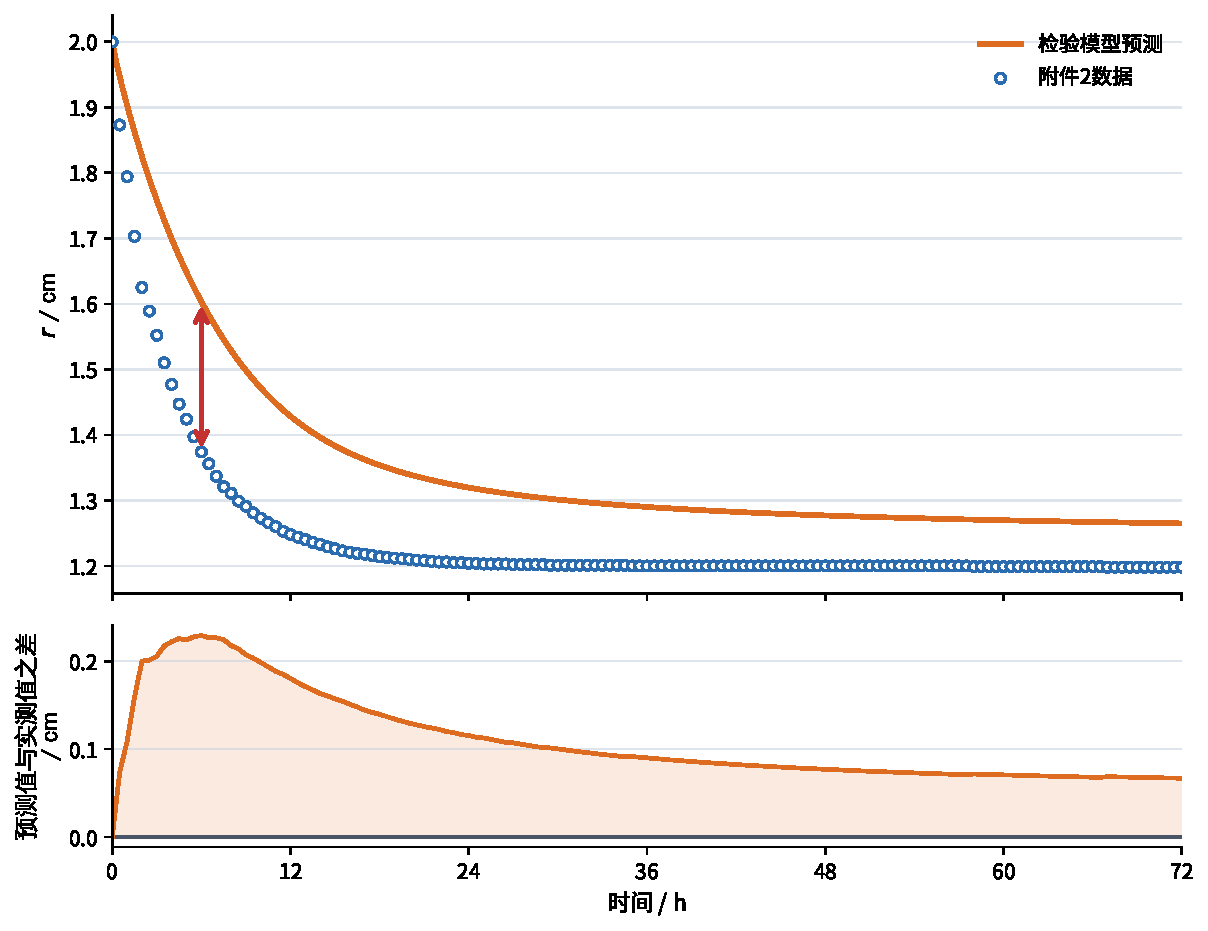
\includegraphics[width=0.90\textwidth]{../../problem4-3/experiments/fixed_length_free_radius_20260911_final/figures/radius_attachment2_comparison.pdf}
\caption{固定长度守恒模型的半径预测与附件2数据}
\label{fig:q4r-radius-comparison}
\end{figure}

两个守恒模型的结果列于表\ref{tab:q4r-comparison}。
\begin{table}[H]
\centering
\small
\renewcommand{\arraystretch}{1.18}
\caption{第四问模型比较}
\label{tab:q4r-comparison}
\begin{tabularx}{\textwidth}{>{\raggedright\arraybackslash}p{0.23\textwidth}>{\centering\arraybackslash}p{0.15\textwidth}>{\raggedright\arraybackslash}X>{\raggedright\arraybackslash}X}
\hline
模型&临界时刻/h&保留条件&检验结果\\
\hline
均匀仿射收缩&51.0906&实测半径、固定长度&干质量检验量下降$10.97\%$\\
实测半径与自由长度&47.8764&真实湿密度、实测半径、干质量守恒&长度最高达到$32.3855\,\mathrm{cm}$\\
固定长度与自由半径&56.2103&真实湿密度、固定长度、干质量守恒&半径RMSE为$0.120537\,\mathrm{cm}$\\
\hline
\end{tabularx}
\end{table}

主模型的空间加密呈二阶收敛，细网格含水率经验误差为$7.25\times10^{-7}\,\mathrm{kg/kg}$；时间加密引起的临界时刻变化为$5.47\times10^{-6}\,\mathrm s$。这些结果支持$51.09\,\mathrm h$的数值稳定性。结合题目要求，第四问采用均匀仿射收缩模型的
\begin{equation}
\boxed{t_4=51.09\,\mathrm h}
\end{equation}
作为计算结果。表\ref{tab:q4r-comparison}中的另两个时长反映几何闭合条件对结果的影响。

% 第四问数值证据：
% ultrafine_runs/fixed_50_005/problem4_final/validation_report.md
% problem4-2/experiments/true_density_nonaffine_20260911_phase3_center_reconstructed/final_validation.md
% problem4-3/experiments/fixed_length_free_radius_20260911_final/结果报告.md

\section{模型评价与展望}

\subsection{模型优点}
\begin{itemize}[leftmargin=2em,itemsep=1pt,topsep=2pt]
  \item 前三问采用统一的径向传热传质框架，模型之间的变化集中在物性、边界时长和几何尺寸。
  \item 第三问通过网格加密和独立算法复算检验临界时刻，第四问通过干质量守恒检验几何闭合条件。
  \item 累计干质量坐标保证每个材料单元的干质量恒定，可直接讨论非均匀收缩。
\end{itemize}

\subsection{模型局限}
\begin{itemize}[leftmargin=2em,itemsep=1pt,topsep=2pt]
  \item 第四问主模型同时采用实测半径和固定长度，按真实湿密度计算时存在干质量偏差。
  \item 长度和孔隙率缺少观测，真实湿密度条件下的几何变形尚未唯一确定。
  \item 一维模型忽略端面附近的轴向梯度，端面传递系数仍需实验标定。
\end{itemize}

\subsection{改进方向}
后续实验可同步记录$R(t)$、$L(t)$和样品质量，并测量代表时刻的体积密度或孔隙率。获得轴向变形数据后，可在累计干质量坐标中加入轴向伸缩比；获得端面传递参数后，可建立二维轴对称$(r,z)$模型。新增观测量将用于确定几何闭合关系，并检验$51.09\,\mathrm h$对收缩机制的敏感程度。
